\documentclass[12pt] {article}
\usepackage{enumerate}
\usepackage{algorithm2e}
\usepackage{mcode}
\usepackage{listings}
\usepackage{graphicx}
\usepackage{epsf}

\author{Zhengwu Zhang}
\title{Homework 3}

\begin{document} 
\maketitle
\newpage
\subsection{Problem 1}

\begin{figure}
\begin{center}
\begin{tabular}{cc}
\includegraphics[height=2.2 in] {prob1f0.eps}
\includegraphics[height=2.2 in] {prob1f.eps}\\
(a) & (b)
\caption{(a)Function of $x^2|sin(\pi x)|e^{-x^3}$. This implies that we could integrate the function from 0 to 3 (b) Density function of $f(x)$}

\end{center}
\end{figure}

\end{document}